\scanpage{143}
\[
(236)\quad
\diagram{\begin{tikzcd}[ampersand replacement=\&,column sep=large]
\deleted{\unsure{D^{*}}}\;\mathcal V^{*}_{D'',Y}\arrow[r]\arrow[d,equal] \& \mathcal V^{*}_{D',Y}\arrow[r]\arrow[d,equal] \& Y\\
\mathcal V_{D'',Y}\setminus\underbrace{\Theta_{D'',Y}}_{\substack{\text{image inverse}\\\text{de }\Theta\text{ sur }\mathcal V_{D'',Y}}} \& \mathcal V_{D',Y}\setminus\Theta_{D',Y} \&
\end{tikzcd}}
\]
\margin{\uline{NB} $\mathcal V^{*}_{D'',Y}$ a la structure du complémentaire d'un diviseur à croisements normaux \inserted{$\Theta''$}, dans un voisinage tubulaire de $\Theta''^{(d_0)*}$ --- et analogue pour $\mathcal V^{*}_{D',Y}$}
\figure{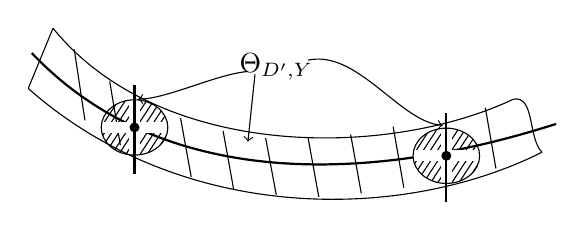
\begin{tikzpicture}[scale=.9]
\draw (-3.3,1.25) .. controls (-1.8,-.6) and (1.4,-.6) .. (3.2,.25);
\draw (-3.65,.4) .. controls (-1.5,-1.5) and (1.6,-1.5) .. (3.6,-.5);
\draw[line width=.8pt] (-3.6,.9) .. controls (-1.7,-1.1) and (1.3,-.9) .. (3.8,-.1);
\draw (-3.3,1.25)--(-3.65,.4);\draw (3.2,.25)..controls(3.5,.3)and(3.4,-.3)..(3.6,-.5);
\foreach \x/\a/\b in {-3/.95/-.05,-2.5/.5/-.4,-1.5/-.02/-.85,-.9/-.2/-1.03,-.3/-.3/-1.1,.3/-.3/-1.13,.9/-.25/-1.08,1.5/-.14/-1,2.8/.13/-.73}{\draw (\x,\a)--(\x+.15,\b);}
\foreach \x/\y in {-2.15/-.15,2.25/-.55}{
\begin{scope}\clip (\x,\y) ellipse (.47 and .39);
\foreach \s in {-1,-.9,...,1}{\draw (\x+\s,\y-.5)--(\x+\s+.65,\y+.5);}
\draw[white,line width=4pt] (\x-.5,\y)--(\x+.5,\y);\draw[white,line width=4pt] (\x,\y-.5)--(\x,\y+.5);
\end{scope}
\draw (\x,\y) ellipse (.47 and .39);\draw[line width=.8pt] (\x,\y-.65)--(\x,\y+.6);\fill (\x,\y) circle(2pt);
}
\node at (-.15,.7) {$\Theta_{D',Y}$};
\draw[->] (-.55,.64)..controls(-1,.6)and(-1.7,.25)..(-2.1,.25);
\draw[->] (-.45,.6)--(-.55,-.35);
\draw[->] (.3,.8)..controls(1,.95)and(1.6,-.08)..(2.2,-.12);
\end{tikzpicture}}

Nous pouvons maintenant définir
\[
(237)\qquad\Pi_1\mathcal V^{*}_{D'',Y}\longrightarrow\Pi_1\mathcal V^{*}_{D',Y}
\]
en définissant les groupoïdes fondamentaux non pas par \inserted{points de} \deleted{base}/\unsure{classes} de chemins, mais par revêtements et isomorphismes entre tels...

C'est en définitive cela, \unsure{l'horreur des|l'heure des} \unsure{normalisations} --- nous pouvons les définir chaque fois qu'on se donne des imm. locales $D''\longrightarrow D'\mathbin{-}Y$
\margin{142}
